% Template for Cogsci submission with R Markdown

% Stuff changed from original Markdown PLOS Template
\documentclass[10pt, letterpaper]{article}

\usepackage{cogsci}


\title{TODO}


\author{{\large \bf Veronica Boyce (vboyce@stanford.edu)} \\ Department of Psychology, \\Stanford University \And {\large \bf TODO (TODO email) } Department of Psychology, \\Stanford University \AND {\large \bf TODO (TODO email)} \\ TODO affiliation, Stanford University \And {\large \bf Michael C. Frank (mcfrank@stanford.edu)} \\ Department of Psychology, \\ Stanford University}


\begin{document}

\maketitle

\begin{abstract}
TODO abstract

\textbf{Keywords:}
TODO keywords
\end{abstract}

\section{Introduction}\label{introduction}

Conversation pacts and partner specificity are often studied by looking
at how they are constructed; an additional perspective comes from how
opaque or interpretable they are to outsiders who weren't part of the
pact

By measuring opaqueness in different conditions related to how the pacts
were formed or what the language looks like, can get another perspective
on the process of pact formation

An empirical test of partner - specificity

Prior work to cover Summary of ref games \& claims around them
(\textbf{hawkins2020b?}) (\textbf{clark1986?}) etc

The side-participant / overhearer etc literature
(\textbf{wilkes-gibbs1992?}), \& lit search for more

Judy's work Visual resemblance and interaction history jointly constrain
pictorial meaning (\textbf{hawkinsb?})

possible could also mention other times when naive comprehender has been
used to better understand iteractive dialogues?

Do we also want to motivate this from a computational angle?
(i.e.~trying to add pragmatics to models) TODO not me

Key question: What properties of conversational pacts and the process of
their formation make them more or less easy for an outsider to
understand?

We use both human experiments and models to assess when and why
expressions are opaque or understandable to outside observers.

Results Figures Conditions/Rounds on accuracy (expt 1+2) (? + model?)
Tangram on accuracy (expt 1+2) (?) (? + model?)

\section{Experimental Methods}\label{experimental-methods}

We ran multiple human experiments that shared methods, so here we
present the general methods, followed by specifics for each experiment.

\subsection{Materials}\label{materials}

TODO discussion of (\textbf{boyce2024?}) and how this is useful

\subsection{Procedure}\label{procedure}

We recruited participants from Prolific (TODO criteria). Participants
were directed to the experiment, where it was explained that previously,
other participants had described these shapes to one another. They would
see a series of transcripts from the prior game, and their task was the
guess what the intended target was. Participants recieved feedback on
whether they were right or wrong on each trial. Participants were
informed that the descriptions could come from different games. TODO
what were the instructions for yoked experiment!. Except when the items
were yoked to an original viewing order, items were shown in a random
order, subject to the constraint that the same target could not repeat
on adjacent trials.

The task was implemented in jsPsych.

\subsection{Experiment 1}\label{experiment-1}

For the first experiment, we primarily wanted to test our methods and
establish a baseline of how well new matchers could do from reading
random transcripts out of order. We did a 2x2 within subjects design,
where we drew the target transcripts from 2 and 6 player games from
Experiment 1 of TODO cite Boyce et al 2024 and from the first and last
blocks of these games. Thus, we would also be able to check whether
early descriptions (before much partner- or group- specific history
could accumulate, but also before a ``good'' description had been
created) or late descriptions (after both history and practice) would be
easier to understand. We recruited XX participants in May 2024 (check)
who each read YY trials (ZZ in each condition).

expt 1 prereg at \url{https://osf.io/k45dr} expt 2 prereg at
\url{https://osf.io/rdp5k}

expts 1 \& 2

tg-matcher 1\& 2 (what veronica ran in May) 1 is 2 and 6 player games,
rounds 1 and 6 in medium thick (60 participants, 60 items each) 2 is 2
and 6 player games, rounds 1 and 6 in thin and thick (60 participants,
64 items each)

\subsection{Experiment 2}\label{experiment-2}

\emph{TODO where should this go, since it's motivated by the results
from expt 1?} After seeing the not big condition differences in
experiment 1, we tried a second experiment drawing from the expt 3 of
Boyce et al in a 2x2x2 within subjects, using the ``thick'' and
``thin'', 2 and 6 person, 1st and last block utterances.

We recruited XX participants in DATE who each read YY trials (ZZ in each
of the 8 conditions).

\subsection{Calibration expt}\label{calibration-expt}

TODO methods

pre-reg at \url{https://osf.io/6pv5e}

modeling approach and selection

how well can models proxy humans? are there differences?

tg-matcher 3 (calibration) 61 participants, 64 items each, from a pool
of 217 transcripts spanning the models full accuracy range

\subsection{Yoked v shuffled}\label{yoked-v-shuffled}

TODO methods pre-reg at \url{https://osf.io/zqwp5}

tg-matcher 4 (SPR + yoked/unyoked) 196 participants (99 in yoked, 97 in
shuffled), each saw all 72 trials from 1 of 10 games. games not chosen
at random

\section{Computational models}\label{computational-models}

Computational methods TODO V doesn't know how to write this QUESTION: do
we focus on mlp pre- or post- calibration?

\section{Results}\label{results}

\subsection{Human accuracy}\label{human-accuracy}

\begin{CodeChunk}
\begin{figure}[t]

{\centering 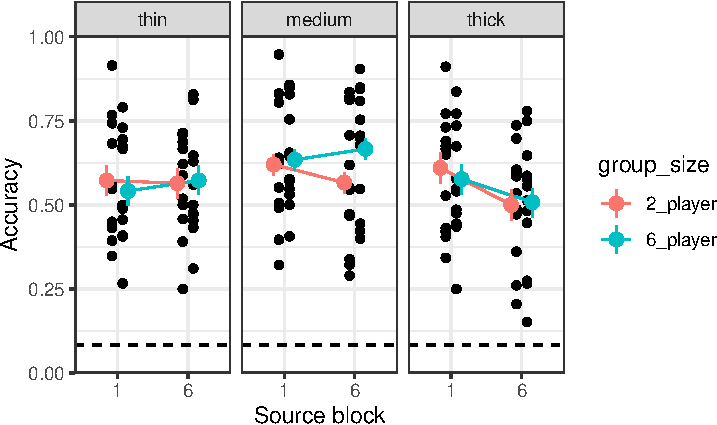
\includegraphics[width=1\linewidth]{figs/fig-1-1} 

}

\caption[TODO We may want to add model predictions onto this as well ]{TODO We may want to add model predictions onto this as well ; may also want to use model predictions b/c error bars don't capture mixed effects \label{TODO}}\label{fig:fig-1}
\end{figure}
\end{CodeChunk}

\begin{CodeChunk}
\begin{figure}[t]

{\centering 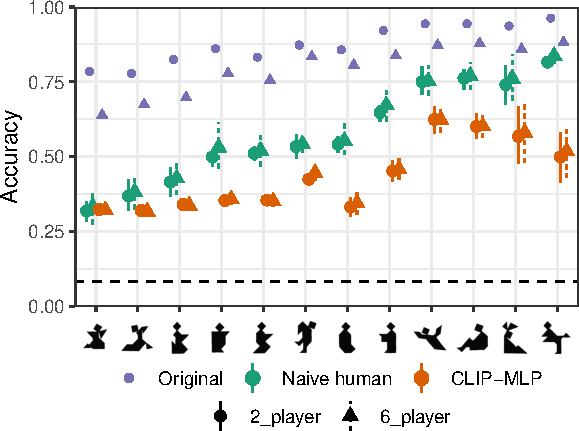
\includegraphics[width=1\linewidth]{figs/fig-2-1} 

}

\caption[TODO We may want to add model predictions onto this as well may also want to use model predictions b/c error bars don't capture mixed effects \label{TODO2}]{TODO We may want to add model predictions onto this as well may also want to use model predictions b/c error bars don't capture mixed effects \label{TODO2}}\label{fig:fig-2}
\end{figure}
\end{CodeChunk}

Expt 1 / 2 : predictors of human accuracy + discussion of high
variability

Expt 1 / 2: (?) model of relationship between original accuracy \& new
matcher accuracy

Expt 1 / 2: (?) adding transcript length as an additional predictor of
human accuracy

what are biggest predictors (conditions, round, target)

Large item level differences, but not a lot else.

TODO will need to extract mixed effects from models into small format
(see mpt for code)

\subsection{Model results (+ calibration
results??)}\label{model-results-calibration-results}

Predictors of model accuracy (what metric?) with some predictors as
above (x3) -- do the same factors that affect human accuracy affect
model accuracy?

predictors of human accuracy + discussion of high variability

model of relationship between original accuracy \& new matcher accuracy

adding transcript length as an additional predictor of human accuracy

(?) What model results to include -- rolling window / anti-rolling / etc
← is there anything good in the what parts of more important stuff (see
incremental-analysis.Rmd, but also all the links broke)

given this proxy -- what can we think we learn -- for instance about
most important parts of the utterances? (rolling window?) does seem to
go up over time

\begin{CodeChunk}
\begin{figure}[t]

{\centering 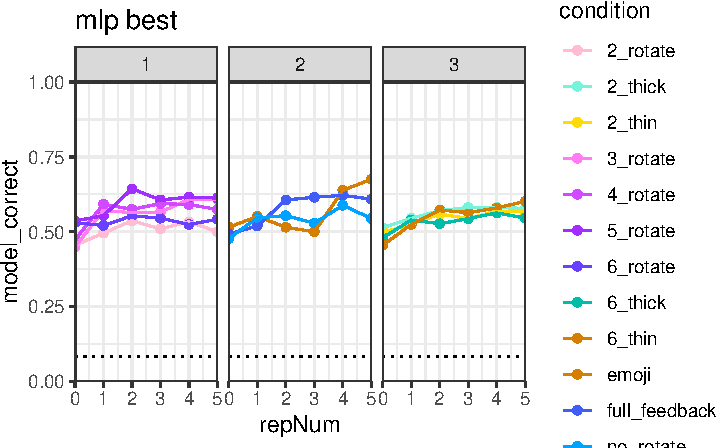
\includegraphics[width=1\linewidth]{figs/fig-4-1} 

}

\caption[Model TODO unclear if this is worth including or in what form, but we do have model on far more than we have human ??]{Model TODO unclear if this is worth including or in what form, but we do have model on far more than we have human ??}\label{fig:fig-4}
\end{figure}
\end{CodeChunk}

TODO not sure what to say re the calibration expt

Numeric results related to calibration ?

TODO ? image related to calibration?

TODO is our ``primary'' model the one pre or post calibration ???

\subsection{Human yoked v not yoked
expt}\label{human-yoked-v-not-yoked-expt}

Yoked v shuffled plot of accuracy (+ model?) Human accuracy on yoked v
shuffled presentation (expt 4) (?) no context model comparison on expt 4
dataset?

seeing things in the same order helps look at item level accuracy
differences?

We will exclude individual word RTs that are greater than 2000 ms.

Condition differences: condition refers to yoked or shuffled. Logistic
model of target selection accuracy: Accuracy \textasciitilde{}
original\_rep\_num * condition + viewing\_order + (1 \textbar{} gameId)
+ (1 \textbar{} tangram) + (1 \textbar{} participant) Time to selection:
Selection\_time \textasciitilde{} original\_rep\_num * condition +
viewing\_order + (1 \textbar{} gameId) + (1 \textbar{} tangram) + (1
\textbar{} participant)

This dataset was collected using a modified self-paced reading
procedure, but for present purposes, we focus only on the selection
results and not on the incremental reading time patterns.

TODO assuming we don't want to include the RT predictor mess here? (and
so not including that whole set of questions)

\begin{CodeChunk}
\begin{figure}[t]

{\centering 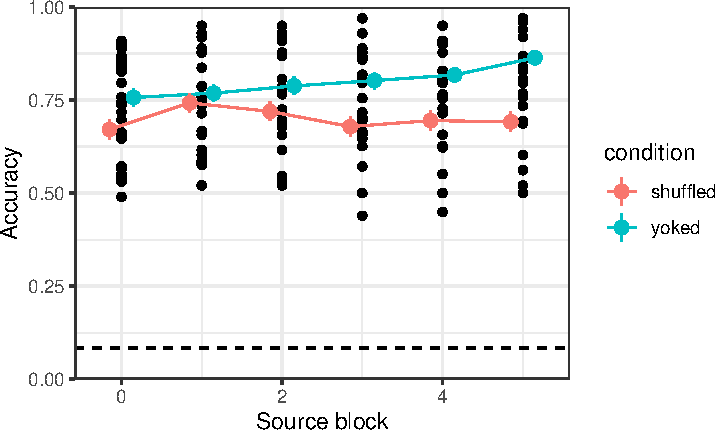
\includegraphics[width=1\linewidth]{figs/fig-n-1} 

}

\caption[TODO also TODO add model comparison ?? \label{yoked}]{TODO also TODO add model comparison ?? \label{yoked}}\label{fig:fig-n}
\end{figure}
\end{CodeChunk}

\section{Discussion}\label{discussion}

Discussion

Understanding varies much more based on item than on anything else;
potentially due to priors or iconicity of image (? that might be beyond
scope -- how well does this match up with say diversity of descriptions)

Models do pretty well? IDK what our model take away is

Especially when there is strong or idiosyncratic reduction, context
helps

role of context

limitations, incuding out of distribution for models

might want to address language comprehension v inference

\section{References}\label{references}

\setlength{\parindent}{-0.1in} 
\setlength{\leftskip}{0.125in}

\noindent

\bibliographystyle{apacite}


\end{document}
